\chapter{Progettazione della didattica}

\section{Le fasi, gli snodi e gli indicatori}

Ogni attività didattica può essere costituita da una o più fasi. Ogni fase a sua volta deve essere svolta secondo uno schema:

\begin{enumerate}
    \item \evidence{consegna}: si introduce la descrizione del compito da svolgere. Deve essere progettato per far emergere dubbi e domande agli studenti;
    \item \evidence{svolgimento}: gli studenti devono svolgere l'attività da soli, in coppia o in gruppo. Il compito dell'insegnante è quello di controllare lo svolgimento della consegna e favorire la discussione;
    \item \evidence{discussione}: ogni studente, coppia o gruppo presenta alla classe la propria soluzione e la discute. Il docente deve far emergere le idee dei singoli. Chiunque presenti una critica a una soluzione deve adeguatamente motivarla;
    \item \evidence{conclusione}: la classe deve essere messa allo stesso livello in base a quanto detto nel punto precedente. L'insegnante si occupa di riassumere i risultati ottenuti.
\end{enumerate}

\nt{La divisione di un'attività in fasi è utile per controllare che ogni studente abbia appreso le competenze necessarie.}

\dfn{Snodi}{Gli \newfancyglitter{snodi} sono i passaggi cognitivi per rispondere correttamente alle domande, svolgere un compito o risolvere un problema.}

\ex{Snodi}{
\begin{itemize}
    \item Comprendere come effettuare una determinata azione;
    \item Eseguire un compito;
    \item Trovare un modo per risolvere un problema.
\end{itemize}
}

\nt{Uno snodo \underline{non è} una fase o una sottofase.}

\dfn{Indicatori}{Gli \newfancyglitter{indicatori} servono per "indicare" se uno snodo è stato superato o meno.}

\ex{Indicatori}{
\begin{itemize}
    \item Frasi;
    \item Domande sulla fase appena svolta;
    \item Commenti sull'attività.
\end{itemize}
}

\section{Obiettivi formativi}

\dfn{Obiettivi formativi}{Gli \newfancyglitter{obiettiv formativi} sono ciò che deve rimanere come apprendimento. Alcune attività possono essere funzionali all'apprendimento in sè pur non avendo contenuti da apprendere.}

\nt{Gli obiettivi dell'insegnamento possono essere \underline{diversi} dagli obiettivi dell'attività.}

\paragraph{Obiettivi formativi:}

\begin{itemize}
    \item \evidence{conoscenze} (K): cosa ci si aspetta che l'alunna conosca dopo l'attività;
    \item \evidence{abilità} (A): cosa ci si aspetta che l'alunno abbia imparato a fare;
    \item \evidence{competenze} (C): come ci si aspetta che l'alunno sappia applicare conoscenze e abilità in un ambiente nuovo, per risolvere un problema.
\end{itemize}

\ex{Obiettivi}{

Lo studente è in grado di $<$verbo di azione$>$ + $<$oggetto$>$ + $[<$specifiche$>]$.
\begin{itemize}
    \item[$\Rightarrow$] Verbo: indica la prestazione attesa. Osservabile e misurabile;
    \item[$\Rightarrow$] Oggetto: la conoscenza che deve essere acquisita;
    \item[$\Rightarrow$] Specifiche: specificano condizioni aggiuntive, tempo, precisione con cui la prestazione deve essere eseguita. Sono opzionali.
\end{itemize}

}

\nt{I verbi non sono casuali, ma sono individuati dalla tassonomia di Bloom}

\dfn{Tassonomia di Bloom}{La \newfancyglitter{tassonomia di Bloom} è un modello di classificazione degli obiettivi educativi che si concentra sui processi cognitivi necessari per completare un compito educativo.}

\nt{La tassonomia di Bloom si articola su più livelli in cui, per proseguire, è necessario aver padroneggiato il piano precedente.}

\begin{center}
    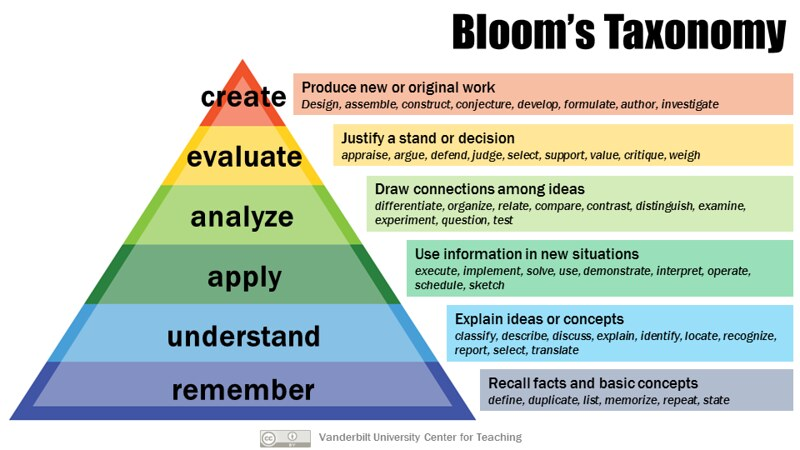
\includegraphics[scale = 0.7]{images/progettazione della didattica/Bloom.jpeg}
\end{center}

\nt{Questa tassonomia va integrata con le indicazioni nazionali, citate in un capitolo precedente.}

\ex{I codici segreti con le vernici}{

\paragraph{Domanda:} come fa un computer a sussurrare il numero di una carta di credito a un altro computer proteggendolo da tutti gli altri computer connessi alla rete?

Per spiegare ciò (lo scambio di chiavi di Diffie-Hellman\footnote{Spiegato in dettaglio nel corso di "Sicurezza"}) si utilizza il trucco delle vernici mescolate:

\begin{itemize}
    \item ognuno ha a disposizione molti colori con nomi precisi;
    \item ognuno ha un set di vernici identico agli altri;
    \item ognuno ha sufficienti barattoli;
    \item ognuno può mescolare le vernici non visto dagli altri.
\end{itemize}

In questo esempio non ci sono comunicazioni segrete, ma solo pubbliche. Il trucco consiste nel fatto che per separare i colori bisogna sapere con quali colori sono formati. Questa è un'attività semplice ma interessante per spiegare il concetto di chiave pubblica e chiave privata.

}






